\chapter{Real-Robot Experiments}

In this chapter, the details of how our experiments are conducted on the real robot are introduced. 
However, due to the complexity of the robot system, the infrastructure built for collecting demonstrations and deploying the neural network policy needs to be described first. Specifically, a real-time system was build to integrate the camera, grippers, whole-body controller, and the VR headset. 

\begin{figure}
	\centering
	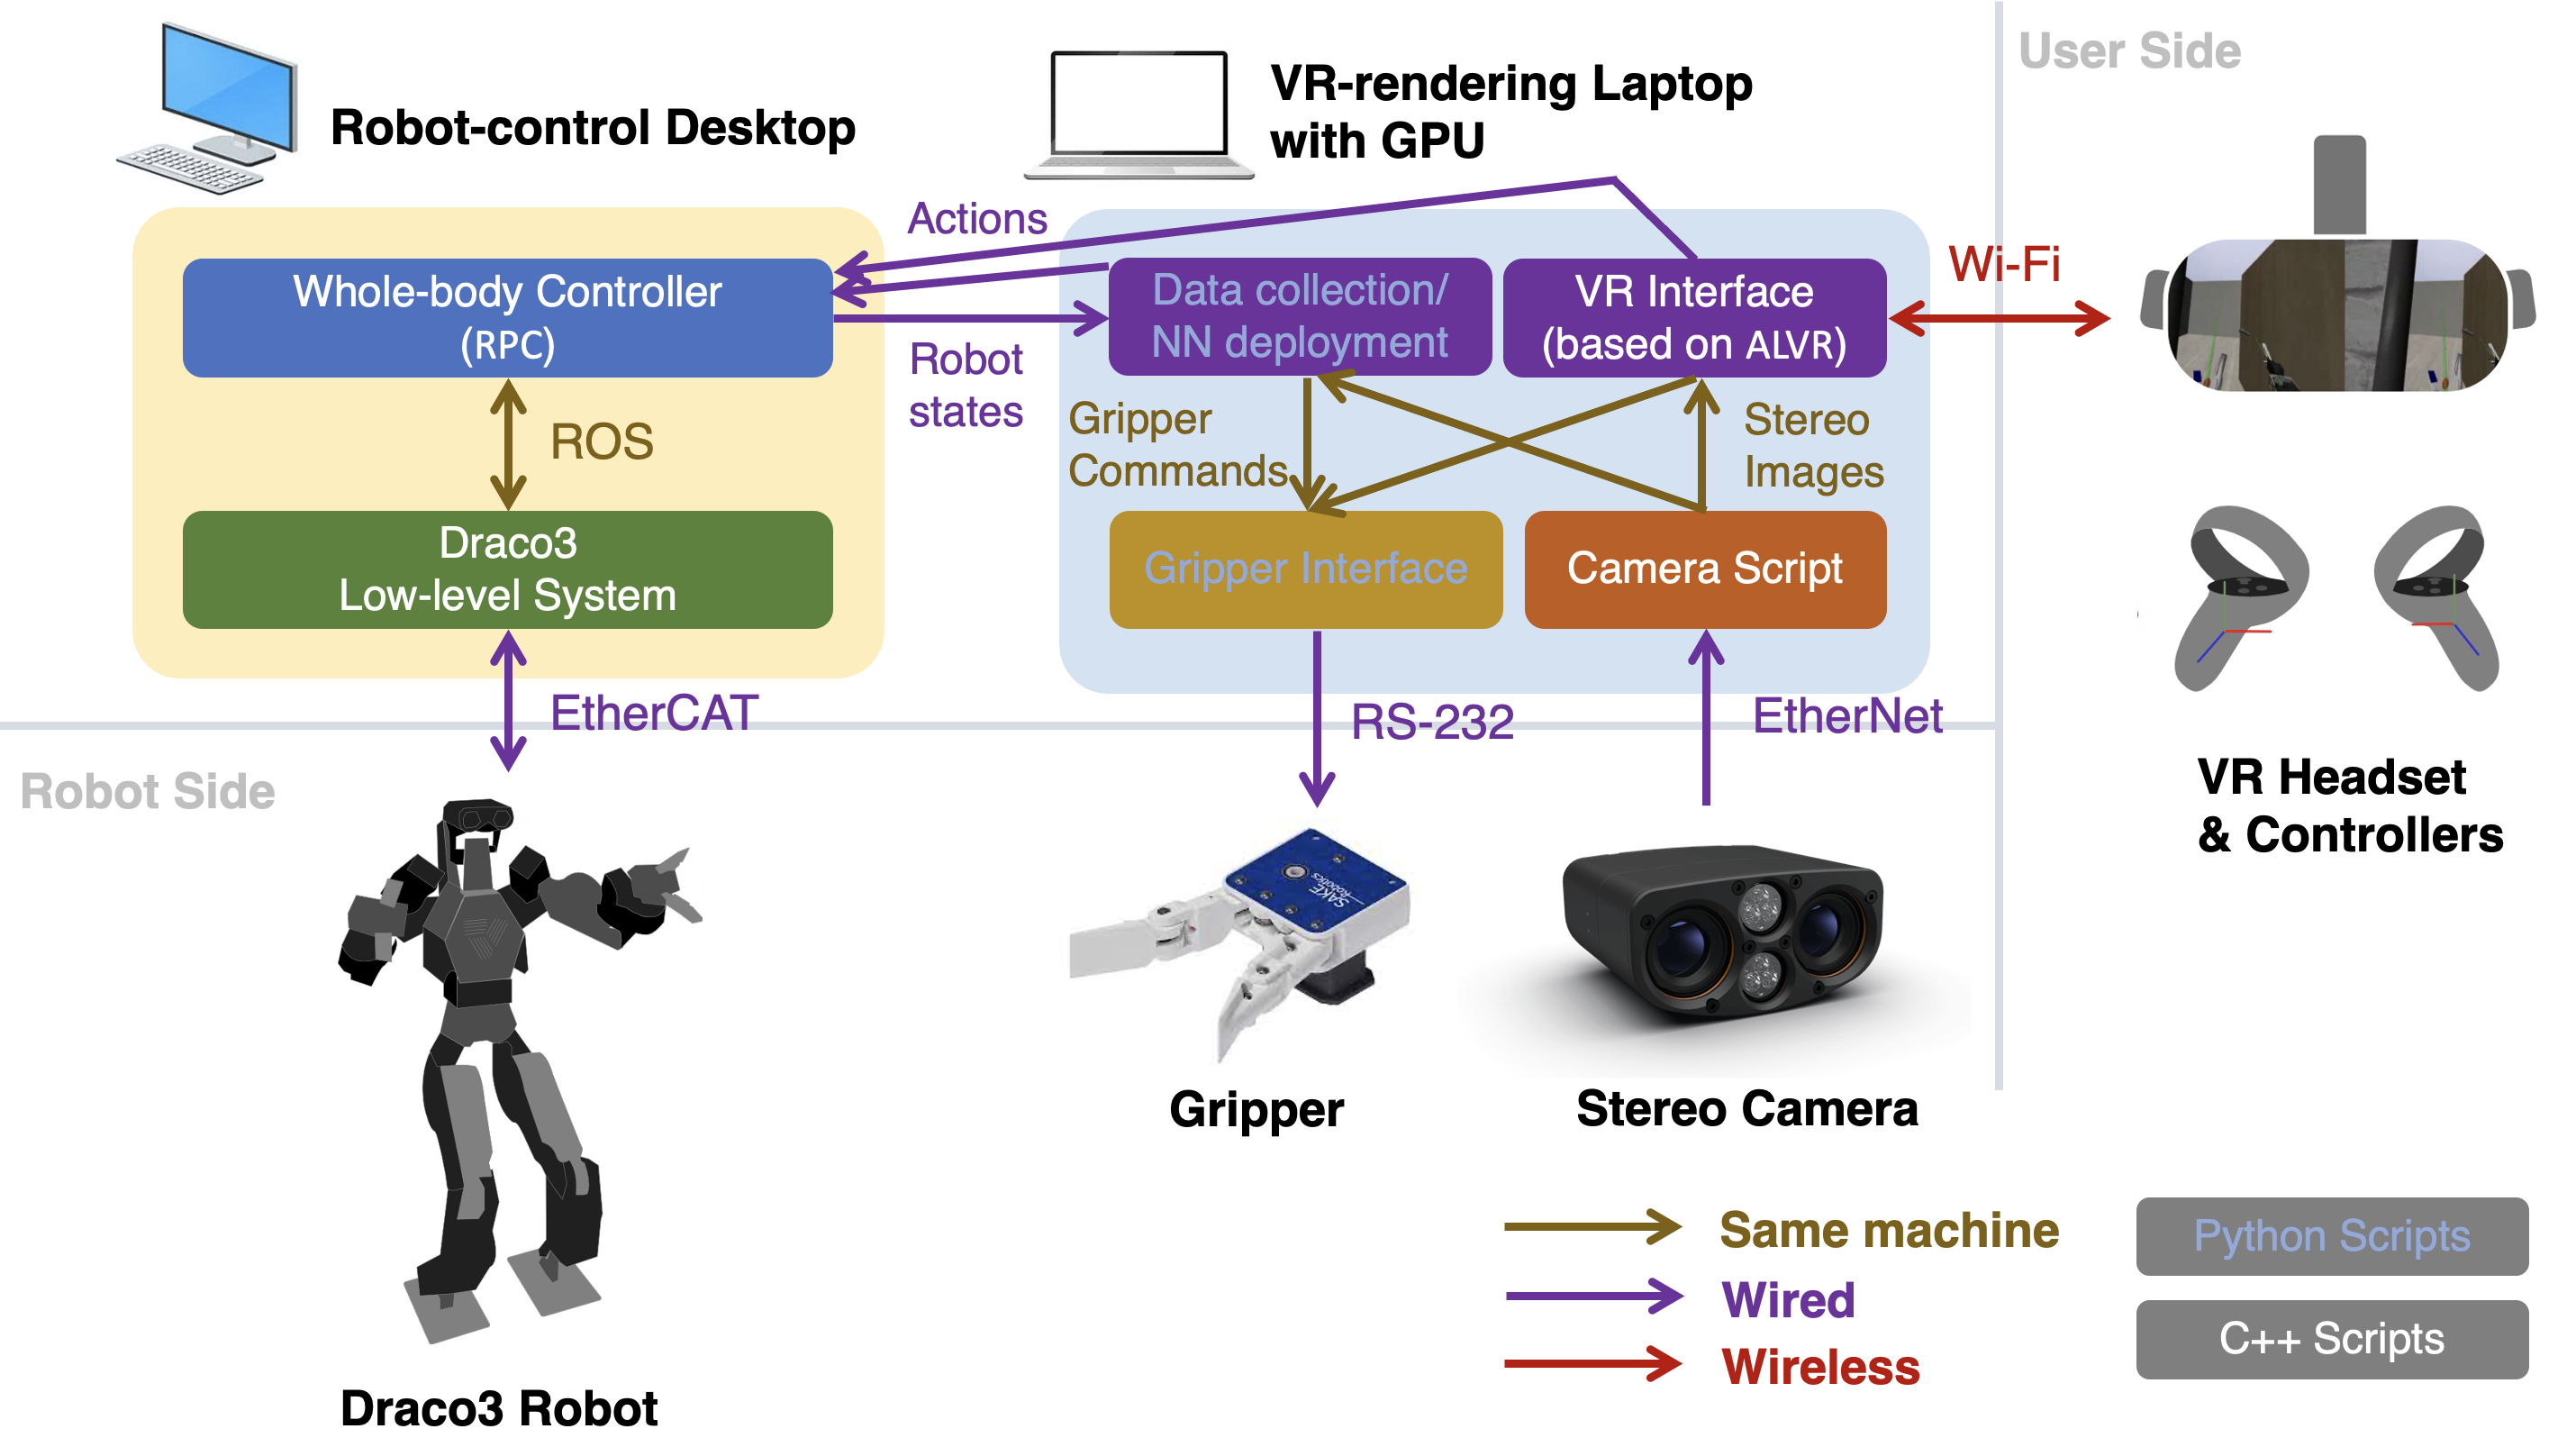
\includegraphics[width=\linewidth]{robot-architecture.png}
	\caption{The infrastructure used to collect demonstraions and deploy policy on the real robot}
    \label{fig:robot-architecture}
\end{figure}


